\documentclass{book} 

\usepackage{graphicx}
\usepackage{amsmath}
\usepackage{algorithm}
\usepackage{algpseudocode}
\usepackage{float}
\usepackage{hyperref}

\hypersetup{
	colorlinks,
	citecolor=black,
	filecolor=black,
	linkcolor=black,
	urlcolor=black
}

\title{Solutions of Introduction to Algorithms}
\author{Saman Saadi}
\date{} 

\begin{document}
	\frontmatter
	\maketitle
%	\newpage
	\tableofcontents
	\mainmatter
	\chapter{Dynamic Programming}
	\section{Rod cutting}
	\subsection{Exercise 2}
	No it cannot always produce an optimal solution. Consider the following example.
	\begin{table}[H]
		\centering
		\begin{tabular}{r||c|c|c}			
			$l_i$ & 1 & 2 & 3\\
			\hline
			$p_i$ & 1 & 50 & 72 \\
			\hline
			$\frac{p_i}{l_i}$ & 1 & 25 & 24
		\end{tabular}
	\end{table}
	For n = 3 the greedy approach cut the rod in 2 pieces. The length of one of them is 2 and the other's is 1. So the profit is $50\$ + 1\$ = 51\$$. But the optimal solution is to keep the rod intact so the profit is $72\$$.
	\subsection{Exercise 3}
	We can keep the rod intact so we don't need to incur the fixed cost c or we can have at least one cut. We need to choose the best solution among all of them:
	\begin{equation*}
	r(i) = \begin{cases}
	\max\limits_{1 \leq k < n}(p_i, r(i - k) + p_k - c) & i > 0 \\
	0 & i = 0
	\end{cases}
	\end{equation*}
	So the solution is $r(n)$. We have n distinct subproblem. In each step we need to choose between keeping the rod intact or have at least one cut which divide the rod into two pieces. The length of one of them is k and the other's $n - k$. We don't know the exact value of k so we need to try all possible values. This can be done in $O(n)$. Therefore the overall running time is $O(n^2)$
	
	\begin{algorithm}
		\begin{algorithmic}[1]
			\Function{f}{p, n, c}
			\State let r[0..n] be a new array
			\State $r[0] \gets 0$
			\For{$\text{j from 1 to n}$}
			\State $q \gets p[j]$
			\For{i from 1 to $j - 1$}
			\State $q = max(q, r[j - i] + p[i] - c)$
			\EndFor
			\State r[j] = q
			\EndFor
			\State \Return $r[n]$
			\EndFunction
		\end{algorithmic}
	\end{algorithm}
	\section{Matrix-chain multiplication}
	\subsection{Exercise 4}
	I've used the following equations:
	\begin{align}
	\sum_{i = 1}^{n} i &= \frac{n(n + 1)}{2}\\
	\sum_{i = 1}^{n} i^2 &= \frac{n(n + 1)(2n + 1)}{6}
	\end{align}
	Each node of the graph represents a distinct sub-problem. Suppose we have two nodes v and u. There is an edge from v to u, if the solution of subproblem v is depended on subproblem u. In other words, there is an edge from m[i, j] to all m[i, k] and m[k + 1, j] for $i \le k < j$. \\
	Usually $|V|$ determines space complexity and $|V| + |E|$ time complexity. we know for every subprobelm m[i, j], $j \ge i$. Hence we have $n - i + 1$ subproblems which starts with $A_i$. So the number of vertices is:
	\begin{equation}
	\begin{split}
	|V| &= \sum_{i = 1}^{n}{n - i + 1} \\
	&= \sum_{i=1}^{n}i \\
	&= \frac{n(n + 1)}{2}
	\end{split}
	\end{equation}
	Hence the space complexity is is $O(n^2)$. We don't use all of the array cells when $j < i$. So we waste $\frac{n^2 - n}{2}$ of allocated array. By analyzing lines 5 - 10 of MATRIX-CHAIN-ORDER pseudocode in the text book we can compute the number of edges.
	\begin{figure}[h!]
		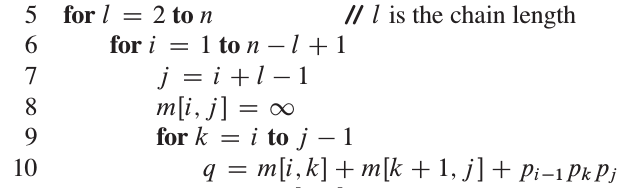
\includegraphics[width=\linewidth]{images/15/15-2-4.png}
		\end{figure}
		As you can see in line 10, m[i, j] is depends on two subproblem m[i, k] and m[k + 1, j]. We visit each distinct subproblem exactly once. So by counting the outdegree of each node we can calculate the number of edges in a directed graph:
		\begin{equation}
		\begin{split}
		|E| &= \sum_{l = 2}^{n}\sum_{i=1}^{n - l + 1}\sum_{k = i}^{i+l-2}2 \\
		&= \sum_{l=2}^{n}\sum_{i=1}^{n-l+1}2(l-1) \\
		&= 2\sum_{l=2}^{n}(n - l + 1)(l-1) \\
		&= 2\sum_{l=2}^{n}(n -(l - 1))(l-1) \\
		&= 2\sum_{l=1}^{n-1}(n-l)l \\
		&= 2(\sum_{l=1}^{n-1}nl - \sum_{l=1}^{n-1}l^2) \\
		&= 2(n\sum_{l=1}^{n-1}l - \sum_{l=1}^{n-1}l^2) \\
		&= 2[n\frac{(n - 1)n}{2} - \frac{(n - 1)(n)(2n - 1)}{6}] \\
		&= n^2(n - 1) - \frac{n(n-1)(2n-1)}{3} \\
		&= \frac{3n^2(n-1)-n(n-1)(2n-1)}{3} \\
		&= \frac{n(n-1)(3n-2n+1)}{3} \\
		&= \frac{n(n-1)(n+1)}{3}\\
		&= \frac{n(n^2-1)}{3}\\
		&= \frac{n^3 - n}{3}
		\end{split}
		\end{equation}
		So the running time is $|V| + |E| = \frac{n^2 + n}{2} + \frac{n^3 - n}{3} = O(n^3)$
		\section{Elements of dynamic programming}
		\subsection{Exercise 2}
		Each node is filled with (p, r). p is the index of leftmost element and r is the index of rightmost element of array which the subprolem wants to sort. As you can see there is no overlapping between subproblems so dynamic programming is not a good idea for merge sort. In other words, we don't see a previously solved subproblem again and we only waste memory. As a general rule if the subproblem graph is a tree, dynamic programming cannot be applied.
		\begin{figure}[h!]
			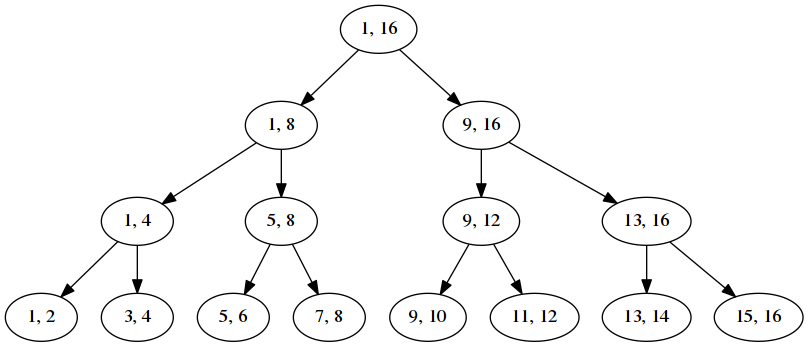
\includegraphics[width=\linewidth]{images/15/15-3-2.png}
		\end{figure}
\end{document}
